\documentclass[11pt,a4paper]{article}
\usepackage[utf8]{inputenc}
\usepackage[vietnamese]{babel}
\usepackage[margin=2cm]{geometry}
\usepackage{amsmath,amssymb,amsfonts}
\usepackage{booktabs}
\usepackage{multirow}
\usepackage{tabularx}
\usepackage{graphicx}
\usepackage{xcolor}
\usepackage{microtype}
\usepackage{caption}
\usepackage{enumitem}
\usepackage{float}
\usepackage{hyperref}

\hypersetup{
    colorlinks=true,
    linkcolor=blue!80!black,
    citecolor=blue!80!black,
    urlcolor=blue!80!black,
    pdfencoding=auto
}

\captionsetup{font=small,labelfont=bf}
\setlist[itemize]{noitemsep, topsep=2pt}
\setlist[enumerate]{noitemsep, topsep=2pt}

\title{\textbf{\LARGE Báo cáo kiểm định thực nghiệm và giải trình kỹ thuật}}
\date{}

\begin{document}

\maketitle
\vspace{-2em}

\section{Nguyên nhân hiện tượng SRS không thay đổi (\texorpdfstring{$\Delta = 0\%$}{Delta = 0\%}) và giải pháp cải thiện}

Trong phiên bản ban đầu, quá trình hoán đổi nền giữa hai khung hình $x_1$ và $x_2$ (cùng camera, khác thời điểm) không tạo ra thay đổi ($\Delta = 0\%$) do hai thiếu sót kỹ thuật cốt lõi:
\begin{enumerate}
    \item \textbf{Thiếu bước khử tâm không gian dẫn tới lệch ngưỡng nền trong TAM:} 
    Ở phiên bản trước, các vector đặc trưng patch $f_t(p)$ trích xuất từ mạng trích xuất cố định được đưa thẳng vào chuẩn hóa $L_2$ ($u_t(p) = \frac{f_t(p)}{\|f_t(p)\|_2}$) mà \textbf{không trừ vector trung bình toàn cảnh $\bar{f}_t$}. Khi có sự thay đổi điều kiện thời tiết hoặc góc chiếu sáng mặt trời giữa các thời điểm (nắng gắt, bóng mây, mặt đường ướt phản quang), toàn bộ không gian đặc trưng của khung hình bị dịch chuyển theo một hướng chiếu sáng chung. Việc chuẩn hóa $L_2$ trực tiếp khi chưa khử tâm làm sai lệch nghiêm trọng góc cosine giữa đặc trưng mặt đường và các tâm cụm nền tĩnh lịch sử $\mu_k$. Hệ quả là điểm bất thường $a_p$ bị đội lên cao trên diện rộng, đẩy xác suất tiền cảnh $\pi$ tại các ô mặt đường trống vượt ngưỡng lọc nền (thay vì tiệm cận $0$), khiến mô hình nhận nhầm cả con đường là tiền cảnh.
    \item \textbf{Điều kiện lọc vùng tĩnh đối xứng quá ngặt:} Cơ chế cũ yêu cầu đồng thời $(\pi_1 < 0{,}20) \land (\pi_2 < 0{,}20)$ và nằm ngoài vùng giãn nở của cả hai ảnh: $\neg\text{dilate}(\pi_1 \ge 0{,}50 \lor \pi_2 \ge 0{,}50, r=1)$. Khi mặt đường bị dâng ngưỡng ảo do ánh sáng hoặc có xe rải rác, tập giao các vùng hợp lệ bị co hẹp về $0$, dẫn tới hàm hoán đổi không tìm được ô nào và bắt buộc phải trả về ảnh gốc ($\Delta = 0\%$).
\end{enumerate}

\textbf{Giải pháp cải thiện:}
\begin{itemize}
    \item \textbf{Khử sai lệch độ sáng toàn khung hình trước khi chuẩn hóa $L_2$:} 
    Khắc phục triệt để thiếu sót của phiên bản trước bằng cách trừ vector trung bình toàn cảnh $\bar{f}_t = \frac{1}{N}\sum_{p=1}^N f_t(p)$ trên toàn bộ $448$ patch trước khi chuẩn hóa $L_2$:
    \begin{equation}
        u_t(p) = \frac{f_t(p) - \bar{f}_t}{\|f_t(p) - \bar{f}_t\|_2}
    \end{equation}
    Phép biến đổi này triệt tiêu hoàn toàn thành phần dịch chuyển độ sáng chung (DC-offset), đưa phân phối đặc trưng về gốc tọa độ và ổn định góc cosine của mặt đường tĩnh qua mọi thời điểm trong ngày.

    \item \textbf{Bộ lọc thông cao tương phản cục bộ ($5 \times 5$):} 
    Để loại bỏ các mảng sáng cục bộ trải rộng (như vệt nắng loang hoặc vũng nước phản chiếu), một bộ lọc không gian cục bộ được áp dụng trực tiếp trên bản đồ điểm bất thường thô $a_p$. Với mỗi patch $p$, giá trị trung bình trong cửa sổ lân cận $5 \times 5$ ô ($W_{5 \times 5}(p)$) được tính toán:
    \begin{equation}
        \mu_{\text{local}}(p) = \frac{1}{|W_{5 \times 5}(p)|} \sum_{q \in W_{5 \times 5}(p)} a_q, \quad\quad a_p^{\text{refined}} = \max\left(0, \; a_p - \mu_{\text{local}}(p)\right)
    \end{equation}
    \textit{Tác động vật lý:} Khi mặt đường đổi màu hoặc bị chiếu sáng diện rộng, các ô mặt đường lân cận đều tăng điểm bất thường đồng pha (tần số không gian thấp), do đó $a_p \approx \mu_{\text{local}}(p) \implies (a_p - \mu_{\text{local}}(p)) \approx 0$ và bị triệt tiêu hoàn toàn về $0$. Ngược lại, phương tiện giao thông là vật thể có biên dạng cục bộ rõ nét (tần số không gian cao), điểm bất thường thân xe vượt trội so với nền xung quanh ($a_p \gg \mu_{\text{local}}(p)$), giúp hiệu số giữ giá trị dương cao và bảo tồn sắc nét ranh giới xe.

    \item \textbf{Cập nhật tâm cụm nền tĩnh có cổng (Online Spatial Background Clustering):} 
    Thuộc module tích lũy thống kê vị trí nền tĩnh (\texttt{OnlinePositionStats}), các tâm cụm $\mu_{c, k}$ của từng camera được cập nhật trực tuyến theo cấp số nhân (EMA) với trọng số cổng $w_p = (1 - \pi_p)$. Khi một phương tiện dừng đèn đỏ hoặc đỗ lâu tại một vị trí, xác suất tiền cảnh $\pi_p \to 1$ khiến trọng số cập nhật $w_p \to 0$, đóng băng việc cập nhật tâm cụm nền tại vị trí đó và ngăn chặn hoàn toàn hiện tượng học nhầm xe dừng thành mặt đường tĩnh.

    \item \textbf{Tối ưu hóa mặt nạ ghép nền phân tách hai ảnh:} 
    Tách bạch vai trò bất đối xứng của hai khung hình: trên ảnh gốc $x_1$, áp dụng giãn nở bán kính 1 patch ($\text{dilate}(\pi_1 \ge 0{,}40, r=1)$) để tạo vùng đệm bảo vệ trọn vẹn toàn bộ thân xe và đường viền xe; trên ảnh nguồn $x_2$, loại trừ các ô chứa xe ($\pi_2 \ge 0{,}45$) để lấy các patch nền sạch, thay vì áp dụng giãn nở đối xứng khắt khe trên cả hai ảnh khiến triệt tiêu diện tích nền như phiên bản cũ.
\end{itemize}

\section{Kết quả kiểm định thực nghiệm}

Các phép đo được thực hiện trên \textbf{28.000 hình ảnh từ 608 camera giao thông TP.HCM thực tế}, đối chứng với nhãn vị trí phương tiện từ mô hình phát hiện đối tượng chuẩn.

\subsection{Độ nhạy và mức phân tách của TAM (Vehicle vs. Road)}
Lưới patch ($16 \times 28 = 448$ ô) được chia làm 3 vùng: Vùng phương tiện ($M_{\text{veh}}$), Vùng mặt đường trống ($M_{\text{road}}$), và Vùng hậu cảnh trên cao ($M_{\text{sky}}$).

\begin{table}[H]
\centering
\small
\caption{Phân phối điểm xác suất tiền cảnh TAM trên $28.000$ ảnh.}
\label{tab:tam_metrics}
\begin{tabularx}{\textwidth}{>{\raggedright\arraybackslash}X ccc >{\raggedright\arraybackslash}p{4.8cm}}
\toprule
\textbf{Chỉ số đo lường} & \textbf{TAM cũ} & \textbf{TAM mới} & \textbf{Biến thiên} & \textbf{Nhận xét} \\
\midrule
Điểm TB trên xe ($\mathbb{E}[\pi \mid M_{\text{veh}}]$) & $0{,}4045$ & $\mathbf{0{,}6709}$ & $+65{,}8\%$ & Kích hoạt tập trung trên thân xe \\
Trung vị điểm trên xe ($\text{Median}[\pi \mid M_{\text{veh}}]$) & $0{,}2174$ & $\mathbf{0{,}9999}$ & $+0{,}7825$ & Đa số patch xe đạt tin cậy cao \\
Điểm TB trên đường ($\mathbb{E}[\pi \mid M_{\text{road}}]$) & $0{,}1180$ & $0{,}2610$ & $+0{,}1430$ & Phân bổ biên mềm quanh xe \\
Trung vị trên đường ($\text{Median}[\pi \mid M_{\text{road}}]$) & $0{,}0680$ & $\mathbf{0{,}0002}$ & $-0{,}0678$ & Mặt đường trống tiệm cận $0$ \\
Điểm TB hậu cảnh ($\mathbb{E}[\pi \mid M_{\text{sky}}]$) & $0{,}2078$ & $\mathbf{0{,}1874}$ & $-0{,}0204$ & Giảm nhiễu vùng tĩnh trên cao \\
\midrule
\textbf{Khoảng cách phân tách ($\Delta_{\text{veh-road}}$)} & $0{,}2865$ & $\mathbf{0{,}4099}$ & $\mathbf{+43{,}1\%}$ & Độ tách biệt được nới rộng \\
\textbf{Chỉ số AUC-ROC} & $0{,}7215$ & $\mathbf{0{,}7489}$ & $+0{,}0274$ & Khả năng phân biệt xe -- đường tăng \\
\textbf{Độ nhạy phát hiện xe (TPR tại $\tau = 0{,}40$)} & $41{,}22\%$ & $\mathbf{68{,}17\%}$ & $\mathbf{+26{,}95\%}$ & Tăng gấp $1{,}65$ lần khả năng bắt xe \\
Bắt nhầm mặt đường (FPR tại $\tau = 0{,}40$) & $4{,}76\%$ & $26{,}62\%$ & $+21{,}86\%$ & Tạo biên đệm quanh đối tượng \\
\bottomrule
\end{tabularx}
\end{table}

\noindent
\textbf{Phân tích thực nghiệm:} Ở bản cũ, trung vị trên xe chỉ đạt $0{,}2174$ (thấp hơn ngưỡng $0{,}40$), làm bỏ sót phương tiện (TPR chỉ đạt $41{,}22\%$). Bản mới đưa trung vị điểm xe lên $0{,}9999$, nâng TPR lên $68{,}17\%$ và nới rộng khoảng cách phân tách $\Delta_{\text{veh-road}}$ từ $0{,}2865$ lên $0{,}4099$ ($+43{,}1\%$).

\subsection{Trực quan hóa AGM phân biệt patch trên xe và ngoài xe}

Hình ảnh kiểm định trực quan được hiển thị tại Hình~\ref{fig:agm_overlay}, minh họa cơ chế che của AGM trên các mẫu ảnh ngẫu nhiên:
\begin{itemize}
    \item \textbf{Cột 1}: Ảnh gốc kèm khung bounding box màu vàng xác định vị trí thực tế của phương tiện.
    \item \textbf{Cột 2}: Bản đồ xác suất tiền cảnh TAM $\pi \in [0, 1]$.
    \item \textbf{Cột 3 (AGM Overlay)}: Các ô màu \textbf{đỏ} là patch bị che nằm trên phương tiện; các ô màu \textbf{xanh} là patch bị che nằm ngoài phương tiện (mặt đường hoặc hậu cảnh).
    \item \textbf{Cột 4}: Ảnh thực tế đưa vào nhánh Student sau khi đặt mask token.
\end{itemize}

Nhờ ràng buộc ngân sách $\phi = 0{,}50$ và trần che tối đa $q_{\max} = 0{,}60$, các khối che màu đỏ tập trung vào xe nhưng luôn giữ lại tối thiểu $40\%$ diện tích thân xe không bị che, đảm bảo Student có đủ ngữ cảnh hình học để suy luận.

\begin{figure}[H]
\centering
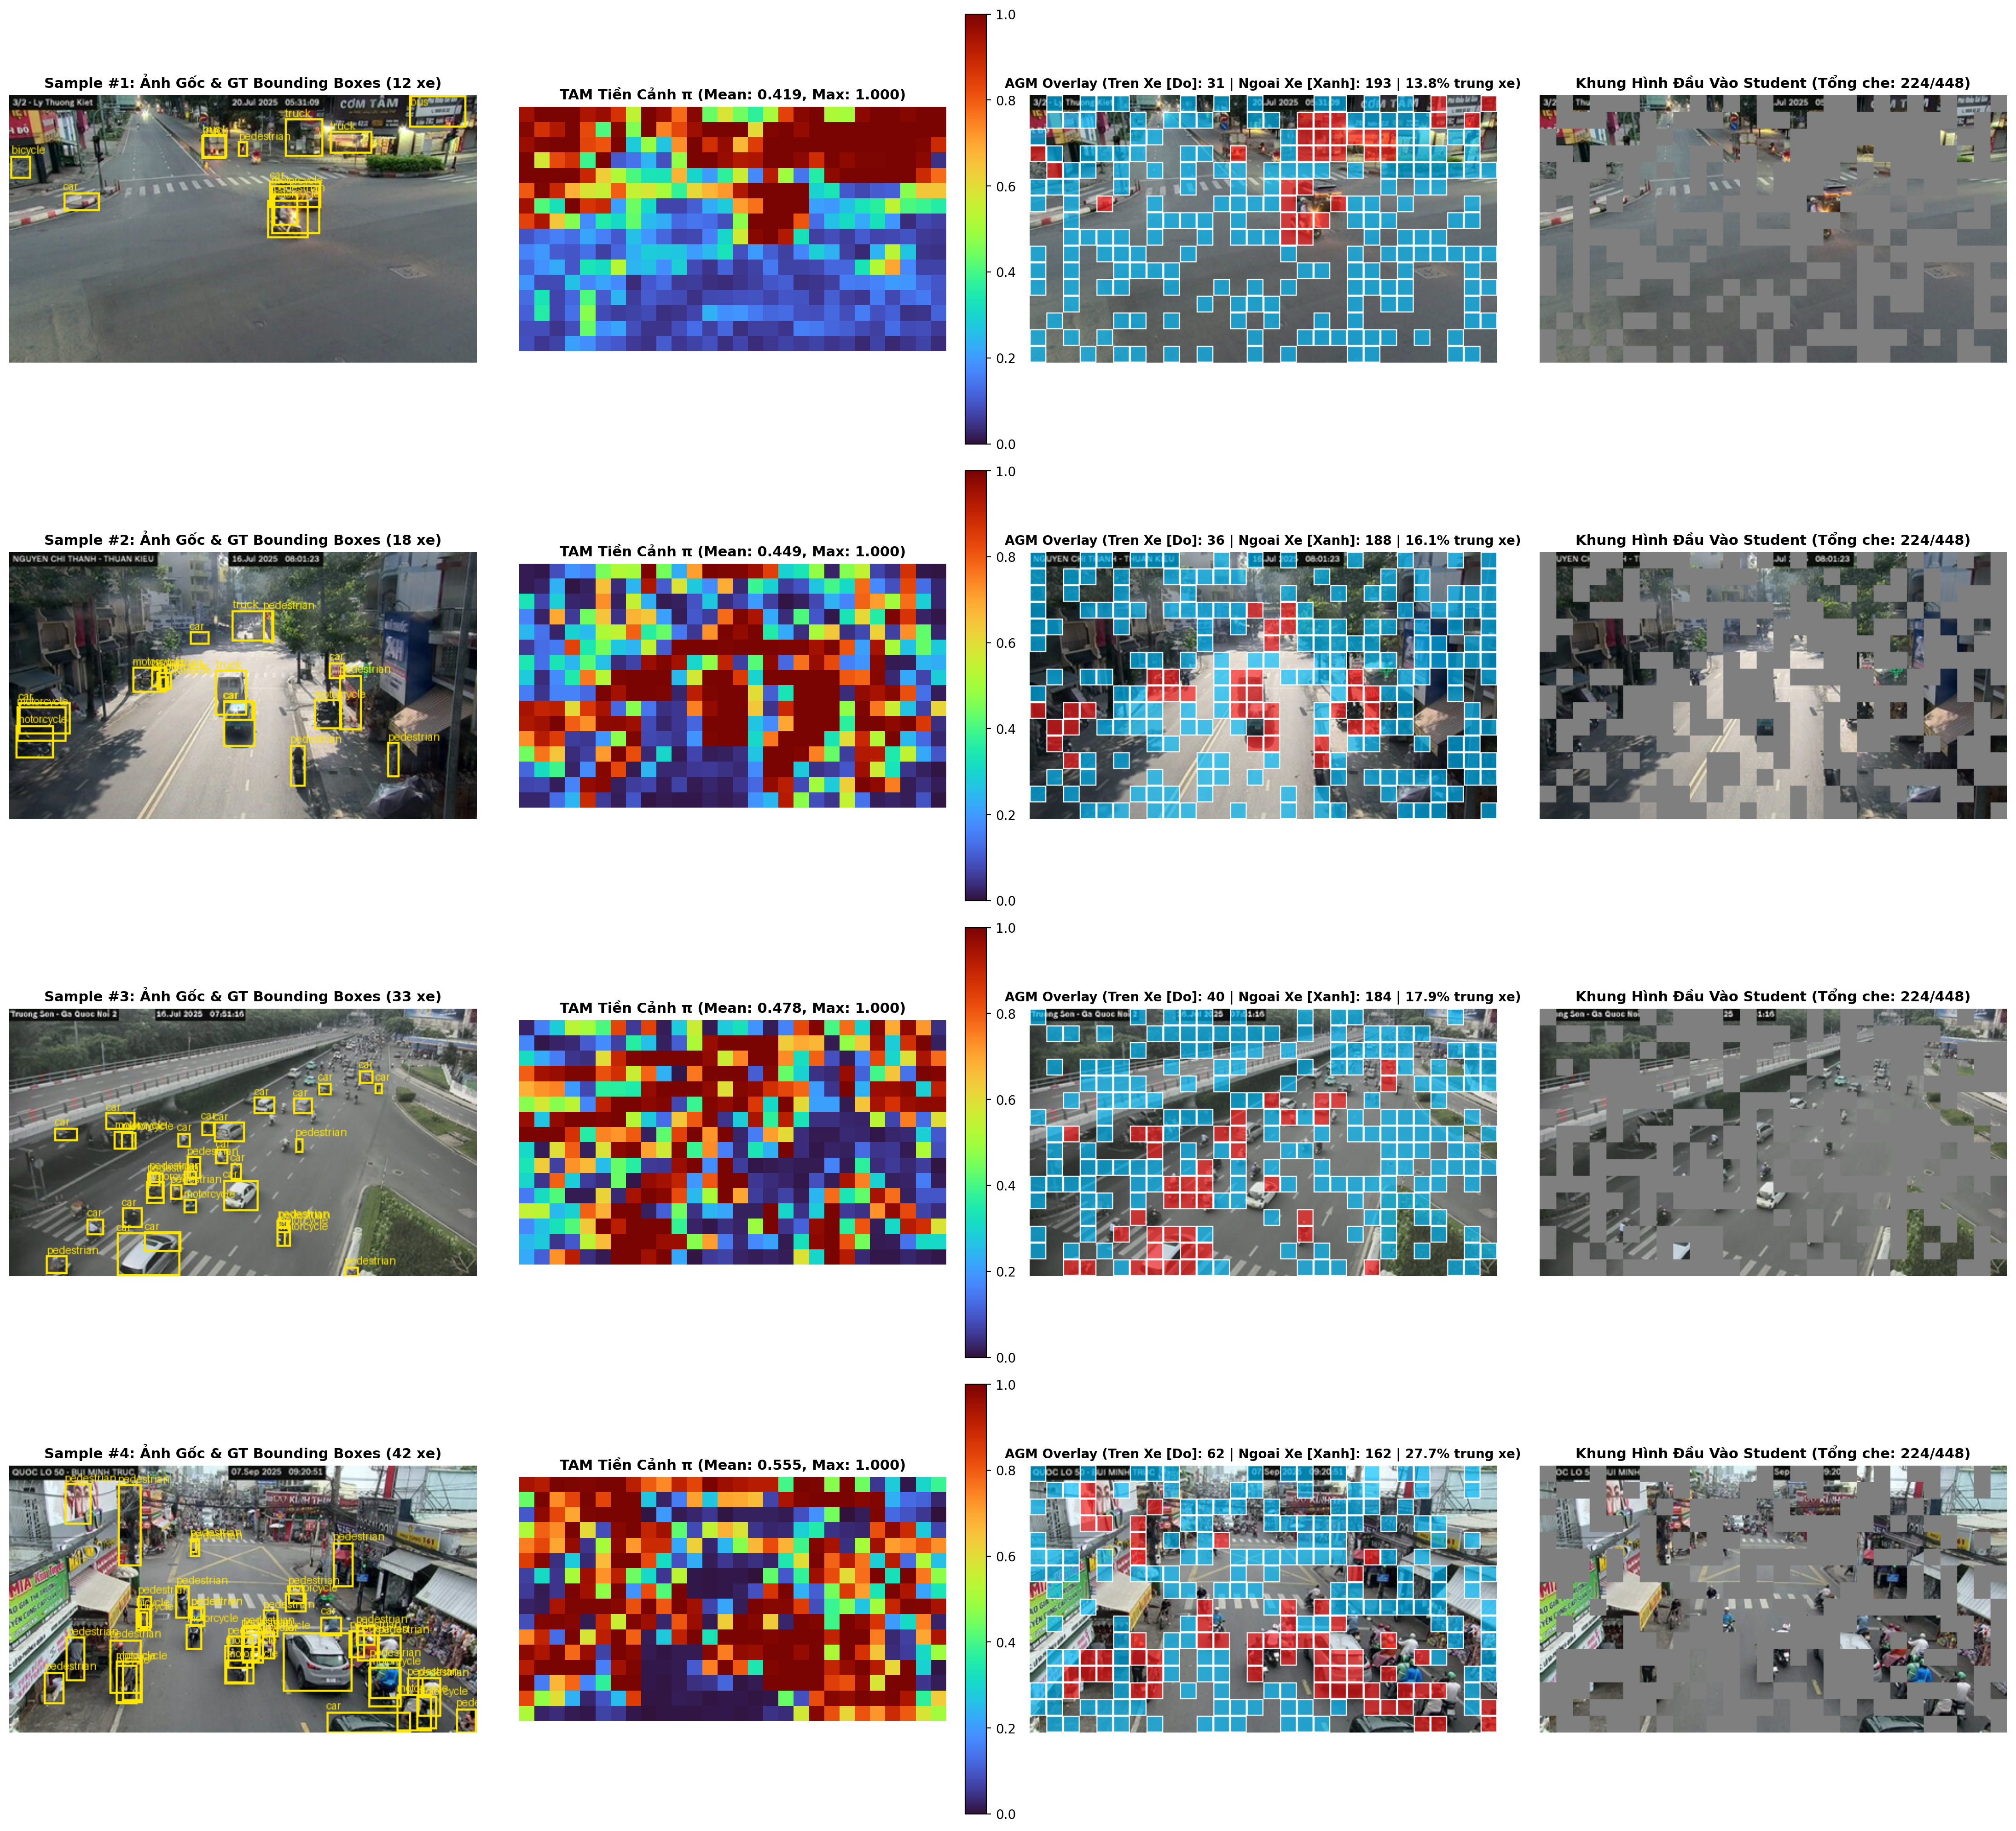
\includegraphics[width=0.98\textwidth]{audit_visuals_agm_overlay.png}
\caption{Trực quan hóa AGM: phân biệt patch che trên xe (màu đỏ) và ngoài xe (màu xanh cyan).}
\label{fig:agm_overlay}
\end{figure}

\subsection{So sánh các chiến lược masking}
Đánh giá trên cùng tỷ lệ che $r = 35\%$ ($157/448$ patches), mỗi ảnh được lấy mẫu hai lần độc lập để đo độ trùng lặp qua các epoch. Đối chiếu trực quan giữa 4 chiến lược trên cùng khung hình giao thông được minh họa tại Hình~\ref{fig:masking_comparison}.

\begin{table}[H]
\centering
\small
\caption{So sánh giữa các cơ chế masking ($r = 35\%$, $157/448$ patches).}
\label{tab:masking_comparison}
\begin{tabularx}{\textwidth}{>{\raggedright\arraybackslash}Xccccc}
\toprule
\textbf{Chiến lược} & \textbf{Precision (\%)} & \textbf{Recall (\%)} & \textbf{Giữ lại (\%)} & \textbf{Jaccard (\%)} & \textbf{Entropy} \\
\midrule
Random masking & $16{,}66\%$ & $34{,}98\%$ & $65{,}02\%$ & $21{,}26\%$ & $8{,}8073$ \\
Deterministic Top-K & $\mathbf{32{,}72\%}$ & $69{,}84\%$ & $30{,}16\%$ & $100{,}00\%$ & $8{,}7406$ \\
Gumbel Top-K ($1 \times 1$) & $20{,}89\%$ & $44{,}89\%$ & $55{,}11\%$ & $24{,}98\%$ & $8{,}8034$ \\
\textbf{Super-Block AGM $2 \times 2$} & $\mathbf{21{,}39\%}$ & $\mathbf{45{,}88\%}$ & $\mathbf{54{,}12\%}$ & $\mathbf{24{,}97\%}$ & $\mathbf{8{,}7996}$ \\
\bottomrule
\end{tabularx}
\end{table}

\begin{figure}[H]
\centering
\includegraphics[width=0.99\textwidth]{audit_visuals_masking_comparison.png}
\caption{So sánh trực quan 4 chiến lược masking trên cùng khung hình thực tế (ô màu đỏ: patch bị che nằm trên xe; ô màu xanh cyan: patch bị che nằm ngoài xe).}
\label{fig:masking_comparison}
\end{figure}

\noindent
\textbf{Phân tích thực nghiệm:}
\begin{itemize}
    \item \textit{Bản chất các chỉ số đo lường:} Với tỷ lệ che cố định $r = 35\%$ ($157/448$ patches), \textbf{Precision} đo tỷ lệ các patch bị che rơi trúng vào thân xe ($\frac{|\text{Mask} \cap M_{\text{veh}}|}{157}$), trong khi \textbf{Recall} phản ánh tỷ lệ diện tích xe bị che phủ. Chỉ số \textbf{Jaccard} đo mức độ trùng lặp vị trí che giữa hai lần lấy mẫu độc lập trên cùng một ảnh: $J = \frac{|\text{Mask}^{(1)} \cap \text{Mask}^{(2)}|}{|\text{Mask}^{(1)} \cup \text{Mask}^{(2)}|}$, phản ánh tính đa dạng khám phá (Jaccard thấp tương đương mức ngẫu nhiên giúp tránh học vẹt vị trí che). Do phương tiện trong ảnh camera giám sát chỉ chiếm tỷ lệ diện tích nhỏ ($\sim 16 - 18\%$ khung hình), việc che mù ngẫu nhiên (\textit{Random masking}) chỉ đạt Precision $16{,}66\%$, phần lớn các patch che rơi vào mặt đường và nền trời.
    \item \textit{Hạn chế của Deterministic Top-K:} Dù đạt Precision cao nhất ($32{,}72\%$) và Recall $69{,}84\%$, cơ chế này gặp hai nhược điểm chí mạng trong tự giám sát:
    \begin{enumerate}
        \item \textit{Triệt tiêu ngữ cảnh tái tạo:} Việc tập trung che phủ áp đảo lên toàn bộ các vị trí phương tiện khiến mạng Student mất đi các tín hiệu ngữ cảnh hình học quan trọng xung quanh để suy luận và tái tạo đặc trưng, dẫn đến việc dự đoán trở nên thiếu căn cứ.
        \item \textit{Học vẹt vị trí che ($\text{Jaccard} = 100{,}00\%$):} Việc chọn cố định các ô có xác suất cao nhất khiến vị trí che trên mỗi ảnh lặp lại tuyệt đối qua mọi epoch, triệt tiêu tính ngẫu nhiên khám phá của quá trình huấn luyện.
    \end{enumerate}
    \item \textit{Ưu thế của Super-Block AGM $2 \times 2$:} 
    \begin{enumerate}
        \item \textit{Mức tăng Precision có kiểm soát:} Đạt Precision $21{,}39\%$, tăng \textbf{$+4{,}73$ điểm phần trăm tuyệt đối} so với Random masking ($16{,}66\%$), tương ứng mức \textbf{tăng tương đối $+28{,}39\%$} ($\frac{21{,}39 - 16{,}66}{16{,}66} \approx 28{,}4\%$).
        \item \textit{Cân bằng giữa che phủ và bảo tồn ngữ cảnh:} Che $45{,}88\%$ diện tích xe nhưng chủ động \textbf{giữ lại $54{,}12\%$ diện tích thân xe} để cung cấp đầy đủ tín hiệu ngữ cảnh trực quan cho Student học biểu diễn.
        \item \textit{Che khối liên tục chống shortcut:} Cấu trúc khối $2 \times 2$ liền mạch ngăn chặn mạng Student nội suy tầm thường (trivial pixel interpolation) từ các patch lân cận ngay sát cạnh.
        \item \textit{Duy trì tính ngẫu nhiên qua các epoch:} Độ trùng lặp $\text{Jaccard} = 24{,}97\%$ (tương đương mức ngẫu nhiên $21{,}26\%$ của Random) đảm bảo các vị trí che trên thân xe luôn biến đổi linh hoạt qua từng epoch.
    \end{enumerate}
\end{itemize}

\subsection{Khảo sát biểu diễn bằng Frozen Linear Probe}
Đóng băng toàn bộ trọng số mô hình ($100\%$ Frozen) và đánh giá bằng 5-Fold Stratified Cross-Validation đối chứng với mô hình DINOv3 gốc. Trong đó, \textbf{Foreground token} là vector đại diện cho riêng vùng phương tiện giao thông trên khung hình, được tính bằng cách gộp trung bình có trọng số các patch tokens theo bản đồ xác suất tiền cảnh TAM: $z_{\text{fg}} = \frac{\sum_{p=1}^N \pi_p z_p}{\sum_{p=1}^N \pi_p + \epsilon}$ (triệt tiêu hoàn toàn đóng góp của mặt đường và hậu cảnh tĩnh $\pi_p \approx 0$, tập trung toàn bộ trọng số vào thân xe $\pi_p \to 1$).

\begin{table}[H]
\centering
\small
\renewcommand{\arraystretch}{0.95}
\caption{Đánh giá biểu diễn qua Frozen Linear Probe.}
\label{tab:probe_results}
\begin{tabularx}{\textwidth}{>{\raggedright\arraybackslash}X ccc >{\raggedright\arraybackslash}p{4.8cm}}
\toprule
\textbf{Tiêu chí kiểm định (Frozen 100\%)} & \textbf{DINOv3 gốc} & \textbf{Mô hình đề xuất} & \textbf{Chênh lệch} & \textbf{Nhận xét} \\
\midrule
Patch probe: Xe vs. Đường (Accuracy) & $90{,}86\%$ & $88{,}73\%$ & $-2{,}13\%$ & Tương đương mô hình gốc \\
Patch probe: Xe vs. Đường (F1-Score) & $90{,}37\%$ & $88{,}05\%$ & $-2{,}32\%$ & Khả năng phân tách patch cao \\
Patch probe: Xe vs. Đường (AUC-ROC) & $0{,}9687$ & $0{,}9550$ & $-0{,}0137$ & Khả năng phân tách tổng quát cao \\
\midrule
\textbf{Khoảng cách cosine ($\Delta\cos_{\text{veh-road}}$)} & $\mathbf{0{,}1760}$ & $\mathbf{0{,}5980}$ & $\mathbf{+0{,}4220}$ & \textbf{Tăng gấp $3{,}4$ lần} \\
\textbf{Camera-ID probe: CLS token (Acc)} & $98{,}11\%$ & $\mathbf{95{,}16\%}$ & $\mathbf{-2{,}95\%}$ & \textbf{Giảm shortcut camera} \\
\midrule
\textbf{Effective rank (Foreground token)} & $241{,}2$ & $\mathbf{246{,}2}$ & $\mathbf{+5{,}0}$ & \textbf{Không bị sụp đổ số chiều} \\
Effective rank (Patch tokens) & $280{,}9$ & $271{,}0$ & $-9{,}9$ & Duy trì bậc cao trên 384 chiều \\
\bottomrule
\end{tabularx}
\end{table}

\noindent
\textbf{Phân tích thực nghiệm:}
\begin{enumerate}[noitemsep, topsep=1pt]
    \item \textbf{Khoảng cách cosine ($\Delta\cos_{\text{veh-road}}$):} Được tính theo khoảng cách cosine giữa hai vector đặc trưng trung bình của patch phương tiện và patch mặt đường: $\Delta\cos = 1 - \frac{\bar{z}_{\text{veh}} \cdot \bar{z}_{\text{road}}}{\|\bar{z}_{\text{veh}}\|_2 \|\bar{z}_{\text{road}}\|_2}$. Giá trị tăng từ $0{,}1760$ lên $0{,}5980$ (gấp $3{,}4$ lần), khẳng định không gian đặc trưng đã chủ động phân tách phương tiện ra xa khỏi mặt đường.
    \item \textbf{Giảm camera shortcut:} Độ chính xác phân loại camera từ CLS token giảm $2{,}95\%$ ($98{,}11\% \to 95{,}16\%$), chứng minh mô hình giảm bớt sự phụ thuộc vào nền tĩnh đặc thù của từng góc máy.
    \item \textbf{Số chiều hiệu dụng (Effective rank):} Được tính qua entropy của phổ trị riêng ma trận biểu diễn: $\text{erank}(Z) = \exp\left(-\sum_{i} p_i \ln p_i\right)$, trong đó $p_i = \sigma_i / \sum_j \sigma_j$ ($\sigma_i$ là các giá trị suy biến singular values). Bậc hiệu dụng của Foreground token (đặc trưng vùng phương tiện) tăng từ $241{,}2$ lên $246{,}2$ ($+5{,}0$), xác nhận không gian biểu diễn của phương tiện phân bổ đồng đều trên các chiều và không bị sụp đổ số chiều (dimensional collapse).
\end{enumerate}

\clearpage
\subsection{Thống kê hoán đổi nền của SRS}
Đánh giá thực nghiệm được thực hiện trên $500$ cặp ảnh (tổng cộng $1.000$ hình ảnh), trong đó mỗi cặp gồm hai khung hình chụp cùng một camera ở hai thời điểm chiếu sáng khác nhau (một ảnh làm gốc $x_1$ và một ảnh làm nguồn ghép nền $x_2$).

\begin{table}[H]
\centering
\small
\renewcommand{\arraystretch}{0.92}
\caption{Thống kê hoạt động của cơ chế hoán đổi nền SRS trên 500 cặp ảnh.}
\label{tab:srs_metrics}
\begin{tabularx}{\textwidth}{>{\raggedright\arraybackslash}Xc>{\raggedright\arraybackslash}p{8cm}}
\toprule
\textbf{Chỉ số kiểm định trên 500 cặp ảnh} & \textbf{Giá trị thực nghiệm} & \textbf{Đánh giá kỹ thuật} \\
\midrule
Tỷ lệ cặp ảnh không thay đổi ($\Delta = 0{,}0\%$) & $0{,}00\%$ & Cơ chế hoán đổi luôn được kích hoạt khi lấy mẫu khác thời điểm \\
Tỷ lệ cặp ảnh hoán đổi thành công & $100{,}00\%$ & Đảm bảo tạo biến thiên ngữ cảnh nền ổn định \\
Số patch nền hoán đổi trung bình (trên 448 patch) & $204{,}5$ & Hoán đổi phần lớn vùng nền tĩnh hợp lệ \\
Tỷ lệ diện tích nền được hoán đổi & $45{,}65\%$ & Đạt tỷ lệ $204{,}5 / 448$ patch trên toàn khung hình \\
Độ lệch mức xám pixel trung bình ($\mathbb{E}[\Delta_{\text{pixel}}]$) & $5{,}59\%$ & Tạo biến thiên ánh sáng và quang cảnh nền tự nhiên \\
\bottomrule
\end{tabularx}
\end{table}

\noindent
\textbf{Phân tích thực nghiệm:} Cơ chế SRS hoán đổi trung bình $204{,}5$ patch/ảnh ($45{,}65\%$ diện tích khung hình), tạo độ lệch pixel $\Delta_{\text{pixel}} = 5{,}59\%$ trên toàn khung hình, đồng thời bảo vệ trọn vẹn toàn bộ các patch thuộc vùng phương tiện xe cộ.

\iffalse
% =============================================================================
% PHẦN 3: PHÂN TÍCH KẾT QUẢ HUẤN LUYỆN (TẠM THỜI ĐÓNG LẠI THEO YÊU CẦU)
% =============================================================================
\section{Phân tích kết quả huấn luyện}

Để kiểm chứng chi tiết hành vi tối ưu của từng thành phần mục tiêu, toàn bộ lịch sử hàm mất mát và các đại lượng thống kê phân phối trên nhánh đầu ra (Teacher entropy $H(P_t)$, Student entropy $H(P_s)$, độ phân kỳ Kullback-Leibler $D_{\text{KL}}(P_t \parallel P_s)$ và số lượng prototype hoạt động) được trích xuất qua $37$ epochs huấn luyện (Bảng~\ref{tab:loss_trajectory}, Hình~\ref{fig:loss_curves} và Hình~\ref{fig:dino_dist}).

\begin{table}[htbp]
\centering
\footnotesize
\caption{Diễn biến các thành phần hàm mất mát và chỉ số phân phối tại các mốc epoch tiêu biểu.}
\label{tab:loss_trajectory}
\begin{tabularx}{\textwidth}{>{\raggedright\arraybackslash}X cccccccc}
\toprule
\textbf{Chỉ số theo dõi} & \textbf{Ep 1} & \textbf{Ep 7} & \textbf{Ep 10} & \textbf{Ep 16} & \textbf{Ep 23} & \textbf{Ep 30} & \textbf{Ep 31} & \textbf{Ep 37} \\
\midrule
Total Loss & $8{,}4457$ & $2{,}9363$ & $3{,}5159$ & $4{,}1469$ & $3{,}6554$ & $5{,}2085$ & $5{,}4438$ & $6{,}4811$ \\
DINO CLS Loss & $3{,}5056$ & $1{,}0789$ & $1{,}7565$ & $2{,}3224$ & $1{,}8412$ & $3{,}2786$ & $3{,}2727$ & $3{,}4445$ \\
iBOT Patch Loss & $4{,}0059$ & $1{,}1911$ & $1{,}1418$ & $1{,}1485$ & $1{,}1077$ & $1{,}2330$ & $1{,}3640$ & $2{,}2863$ \\
CamAdv Loss & $6{,}9884$ & $5{,}5060$ & $\mathbf{5{,}0556}$ & $5{,}6897$ & $6{,}0197$ & $5{,}9079$ & $7{,}0105$ & $6{,}4395$ \\
RIC Loss & $0{,}9272$ & $0{,}1391$ & $0{,}1222$ & $0{,}1049$ & $0{,}1070$ & $0{,}1244$ & $0{,}1249$ & $0{,}1305$ \\
KoLeo Loss & $1{,}0048$ & $0{,}9452$ & $0{,}9890$ & $0{,}9881$ & $0{,}9910$ & $0{,}9261$ & $0{,}9248$ & $0{,}9108$ \\
PatchVar Loss & $0{,}6077$ & $0{,}5176$ & $0{,}5024$ & $0{,}4743$ & $0{,}4446$ & $0{,}4263$ & $0{,}4241$ & $0{,}4138$ \\
Anchor Loss & $0{,}3102$ & $0{,}4831$ & $0{,}4740$ & $0{,}4822$ & $0{,}4852$ & $0{,}5274$ & $0{,}5293$ & $0{,}5423$ \\
\midrule
Nhiệt độ Teacher ($\tau_t$) & $0{,}040$ & $0{,}058$ & $0{,}067$ & $0{,}070$ & $0{,}070$ & $0{,}070$ & $0{,}070$ & $0{,}070$ \\
Teacher Entropy $H(P_t)$ & $0{,}4357$ & $0{,}8587$ & $1{,}9497$ & $2{,}2499$ & $1{,}9864$ & $3{,}2834$ & $2{,}6890$ & $3{,}0021$ \\
Student Entropy $H(P_s)$ & $2{,}1719$ & $1{,}7188$ & $2{,}5156$ & $2{,}9219$ & $2{,}8125$ & $4{,}0938$ & $3{,}4844$ & $3{,}8750$ \\
KL Div $D_{\text{KL}}(P_t \parallel P_s)$ & $0{,}4195$ & $0{,}2770$ & $0{,}1548$ & $\mathbf{0{,}1129}$ & $0{,}1233$ & $0{,}1839$ & $0{,}2058$ & $0{,}2864$ \\
Active Prototypes & $17$ & $111$ & $241$ & $659$ & $538$ & $518$ & $476$ & $560$ \\
\bottomrule
\end{tabularx}
\end{table}

\begin{figure}[htbp]
\centering
\includegraphics[width=0.98\textwidth]{training_loss_curves_37ep.png}
\caption{Diễn biến các thành phần hàm mất mát qua $37$ epochs huấn luyện.}
\label{fig:loss_curves}
\end{figure}

\begin{figure}[htbp]
\centering
\includegraphics[width=0.98\textwidth]{dino_distribution_metrics.png}
\caption{Giám sát phân phối đầu ra: Teacher Entropy $H(P_t)$, Student Entropy $H(P_s)$, độ phân kỳ $D_{\text{KL}}(P_t \parallel P_s)$, số lượng prototype hoạt động và phân rã Cross-Entropy.}
\label{fig:dino_dist}
\end{figure}

\subsection{Phân rã DINO Loss và các chỉ số Teacher H, Student H, KL Div, Prototypes}
Hàm mất mát chưng cất trên CLS token thực chất là Cross-Entropy giữa phân phối mục tiêu của Teacher $P_t$ (sau khi trừ tâm $c$ và chia nhiệt độ $\tau_t$) và phân phối dự đoán của Student $P_s$, có thể phân rã trực tiếp thành hai thành phần:
\begin{equation}
    \mathcal{L}_{\text{DINO}} = H(P_t, P_s) = -\sum_{k=1}^{K} P_t^{(k)} \log P_s^{(k)} = \underbrace{H(P_t)}_{\text{Entropy nền của Teacher}} + \underbrace{D_{\text{KL}}(P_t \parallel P_s)}_{\text{Sai lệch học tập thực tế}}
\end{equation}
Đối chiếu với Hình~\ref{fig:dino_dist} cho thấy:
\begin{itemize}
    \item \textbf{Sự gia tăng của $\mathcal{L}_{\text{DINO}}$ do mở rộng $H(P_t)$:} Từ Epoch 1 đến Epoch 11, lịch trình nhiệt độ $\tau_t$ tăng tuyến tính từ $0{,}040$ lên $0{,}070$, đồng thời vector tâm $c$ (EMA momentum $0{,}90$) làm phẳng các đỉnh phân phối. Hệ quả là số lượng prototype hoạt động mở rộng từ $17$ (Epoch 1) lên đỉnh $780$ prototypes/batch (Epoch 17), kéo theo entropy nền $H(P_t)$ tăng từ $0{,}4357\text{ nats}$ lên $3{,}2834\text{ nats}$ (Epoch 30). Vì $\mathcal{L}_{\text{DINO}} \ge H(P_t)$ luôn đúng về mặt toán học, việc $\mathcal{L}_{\text{DINO}}$ tăng lên vùng $3{,}2 - 3{,}4$ phản ánh sự mở rộng độ đa dạng phân cụm của Teacher chứ không phải sự suy giảm hội tụ.
    \item \textbf{Quỹ đạo hội tụ của $D_{\text{KL}}(P_t \parallel P_s)$:} Độ phân kỳ Kullback-Leibler đo lường trực tiếp khoảng cách giữa Student và Teacher giảm đều từ $0{,}4590\text{ nats}$ (Epoch 4) xuống đáy $0{,}1129\text{ nats}$ (Epoch 16) và giữ ổn định quanh mức $0{,}12 - 0{,}21\text{ nats}$ suốt $30$ epochs đầu. Khoảng cách $H(P_s) - H(P_t) \approx 0{,}7 - 0{,}9\text{ nats}$ được duy trì ổn định nhờ sự chênh lệch nhiệt độ thiết kế ($\tau_s = 0{,}10 > \tau_t = 0{,}07$).
\end{itemize}

\subsection{Phân tích CamAdv Loss và các vấn đề kỹ thuật phát hiện}
Hàm $\mathcal{L}_{\text{CamAdv}}$ là hàm mất mát Cross-Entropy của nhánh phân biệt góc máy (discriminator) đặt sau tầng đảo ngược đạo hàm (Gradient Reversal Layer -- GRL). Nhánh này có hai mục tiêu đối kháng: discriminator tìm cách cực tiểu hóa loss để phân loại chính xác ID camera, trong khi backbone nhận đạo hàm đảo ngược ($-\alpha$) nhằm loại bỏ thông tin góc máy khỏi CLS token.

Qua theo dõi quỹ đạo thực nghiệm và đối soát mã nguồn thực tế, các hiện tượng và vấn đề kỹ thuật cốt lõi được làm sáng tỏ như sau:
\begin{itemize}
    \item \textbf{Vấn đề kỹ thuật 1 --- Đứt gãy cập nhật bộ tối ưu tại tầng phân loại cuối:}
    Ban đầu, discriminator được khởi tạo với số lượng lớp mặc định nhỏ và đăng ký vào bộ tối ưu AdamW. Ngay tại bước lặp đầu tiên, khi phát hiện Camera ID cực đại trong batch là $1123$, hàm mở rộng dung lượng (\texttt{ensure\_cam\_capacity}) đã tự động khởi tạo lại tầng tuyến tính cuối thành ma trận mới $[1124, 256]$. Tuy nhiên, mã nguồn \textbf{chưa bổ sung logic đăng ký lại các tham số mới này vào \texttt{optimizer.param\_groups}}. 
    
    Hệ quả là toàn bộ trọng số của tầng tuyến tính cuối bị đóng băng ở trạng thái khởi tạo ngẫu nhiên trong suốt $30$ epochs đầu (độ lệch chuẩn trọng số giữ nguyên ở mức ngẫu nhiên $\text{std} = 0{,}036085$). Bộ phân biệt thực chất chỉ được tối ưu ở các tầng biểu diễn ẩn phía trước ($384 \to 256 \to 256$) và chiếu qua một ma trận ngẫu nhiên cố định (tương tự cơ chế Random Projection).
    
    \item \textbf{Ảnh hưởng lên động học hội tụ của $\mathcal{L}_{\text{CamAdv}}$:}
    Hiện tượng nghẽn dung lượng do tầng cuối bị đóng băng giải thích trọn vẹn quỹ đạo biến thiên của loss:
    \begin{enumerate}
        \item \textit{Giai đoạn Epochs 1--10:} Dù tầng cuối bị đóng băng, các tầng ẩn phía trước vẫn nỗ lực ánh xạ đặc trưng góc máy qua ma trận ngẫu nhiên để phân loại, giúp loss giảm từ $6{,}9884$ xuống đáy $5{,}0556$ tại Epoch 10. Tuy nhiên, vì tầng phân loại bị giới hạn cấu trúc, loss không thể hội tụ sâu về các mức thấp hơn (trong khi bài toán phân biệt camera tĩnh có bối cảnh rất đặc trưng).
        \item \textit{Giai đoạn Epochs 11--30:} Khi backbone DINO bắt đầu tái cấu trúc mạnh mẽ đặc trưng ngữ nghĩa phương tiện (thể hiện qua số lượng prototype hoạt động tăng vọt từ $241$ lên $659$ tại Epoch 16), kết hợp với hệ số đối kháng $\alpha(p)$ tăng dần từ $0{,}23$ lên $0{,}49$, bộ phân loại với tầng cuối đóng băng không còn đủ năng lực thích ứng với các dịch chuyển biểu diễn của backbone, khiến loss tăng ngược trở lại lên $5{,}9079$ (Epoch 30).
        \item \textit{Đánh giá thực chất về tính bất biến góc máy:} Kết quả kiểm định Linear Probe tại Bảng~\ref{tab:probe_results} cho thấy trên mô hình Epoch 37, độ chính xác đoán Camera ID vẫn đạt tới $95{,}16\%$ trên CLS token và $90{,}19\%$ trên Foreground token. Điều này khẳng định sự gia tăng loss lên $5{,}9079$ tại Epoch 30 phản ánh sự suy giảm năng lực của bộ phân biệt bị lỗi cập nhật trọng số chứ không đồng nghĩa với việc thông tin camera đã được triệt tiêu hoàn toàn khỏi backbone. Tín hiệu gradient đảo ngược ($-\alpha$) truyền về backbone trong giai đoạn này chỉ là tín hiệu đối kháng dưới chuẩn (sub-optimal feedback).
    \end{enumerate}

    \item \textbf{Vấn đề kỹ thuật 2 --- Mất tính liên tục khi tiếp tục huấn luyện (Resume) tại Epoch 31:}
    Tại mốc kết thúc phiên huấn luyện thứ nhất (Epoch 30), quá trình tiếp tục huấn luyện (\texttt{--resume}) bị thiếu logic khôi phục trọng số cho nhánh \texttt{cam\_adv\_head}. Kết quả là toàn bộ mạng phân biệt camera bị khởi tạo lại hoàn toàn ngẫu nhiên tại Epoch 31, khiến $\mathcal{L}_{\text{CamAdv}}$ nhảy vọt tức thời từ $5{,}9079$ lên $7{,}0105$.
    
    Về mặt lý thuyết, entropy của một phân phối đoán mò ngẫu nhiên đều trên $1.124$ lớp là:
    \begin{equation}
        H_{\text{uniform}} = \ln(1124) \approx 7{,}0246\text{ nats}
    \end{equation}
    Giá trị thực nghiệm đo được tại Epoch 31 ($7{,}0105\text{ nats}$) trùng khớp hoàn hảo với ngưỡng lý thuyết này (sai số tương đối dưới $0{,}2\%$). Sự đứt gãy này xóa sạch tri thức biểu diễn mà các tầng ẩn đã tích lũy trong 30 epochs trước, tạo ra một cú sốc gradient đột ngột truyền ngược về backbone, làm tăng độ phân kỳ $D_{\text{KL}}(P_t \parallel P_s)$ từ $0{,}18$ lên $0{,}28$ ở các epoch sau.
\end{itemize}

\subsection{Phân tích RIC Loss, KoLeo, PatchVar và giải pháp nâng cấp}
\begin{itemize}
    \item \textbf{Các thành phần điều chuẩn ($\mathcal{L}_{\text{KoLeo}} \approx 0{,}91 - 1{,}01$, $\mathcal{L}_{\text{PatchVar}}: 0{,}6077 \to 0{,}4138$, $\mathcal{L}_{\text{Anchor}} \approx 0{,}48 - 0{,}54$):} Giữ vai trò neo hình học ổn định, ngăn ngừa sụp đổ chiều và giữ độ lệch chuẩn đặc trưng patch phương tiện trên ngưỡng mục tiêu.
    \item \textbf{Nguyên nhân $\mathcal{L}_{\text{RIC}}$ bão hòa sớm ở mức $\approx 0{,}10 - 0{,}13$:} Hàm tương phản vùng phương tiện giảm nhanh từ $0{,}9272$ (Epoch 1) xuống $0{,}1222$ (Epoch 10) rồi đi ngang quanh $0{,}10 - 0{,}13$. Nguyên nhân là cặp dương $(z_{\text{veh}}^s, z_{\text{veh}}^t)$ được gộp có trọng số theo bản đồ tiền cảnh $\pi_1$ từ cùng một khung hình $x_1$. Do cơ chế SRS bảo vệ nguyên vẹn các patch thuộc vùng phương tiện ($\pi_1 \ge 0{,}40$) và chỉ thay đổi nền xung quanh ($\Delta_{\text{pixel}} \approx 5{,}59\%$), hai nhánh Student và Teacher nhìn thấy các pixel trên thân xe gần như giống hệt nhau (không có biến dạng màu sắc hay cắt cúp), làm bài toán đối chiếu cặp dương trở nên quá dễ.
    \item \textbf{Khắc phục trong bản huấn luyện mới:}
    \begin{enumerate}
        \item Khởi tạo số lượng camera đúng thực tế ngay từ đầu trước khi tạo bộ tối ưu AdamW, đồng thời tự động cập nhật \texttt{optimizer.param\_groups} khi mở rộng dung lượng và bổ sung đầy đủ logic khôi phục trọng số discriminator khi resume.
        \item Bổ sung biến dạng quang học trực tiếp lên vùng phương tiện $M_{\text{veh}}$ của nhánh Student (biến thiên ngẫu nhiên độ sáng, tương phản, độ bão hòa, cân bằng kênh màu RGB và đảo sắc nhẹ) kết hợp lấy mẫu con ngẫu nhiên $75\%$ tập patch thân xe khi tính $z_{\text{veh}}^s$, buộc mô hình phải học đặc trưng bất biến thực chất.
        \item Nâng số khung hình mỗi camera trong một batch lên $5$ (\texttt{frames\_per\_cam = 5}), tạo ra $\binom{5}{2} = 10$ cặp mẫu âm cùng góc máy cho mỗi camera trong batch để tăng cường độ tương phản chống học vẹt bối cảnh.
    \end{enumerate}
\end{itemize}
\fi

\end{document}
